\documentclass{udpreport}
%\headertext{Metodos Numéricos}
\title{Retirement Simulator\\
Proyectos en TICS I}
\author{\\[2cm]Javiera Araya, Camilo Araya. \\[1cm]Profesor: Jorge Elliot}
\usepackage{amssymb}
\usepackage{amsmath}
\usepackage{graphicx}
\usepackage{float}
\usepackage{subfig}
\usepackage{array}
\graphicspath{ {Imagenes/} }
\usepackage{listings}
\usepackage{color}
\providecommand{\norm}[1]{\lVert#1\rVert}

\definecolor{dkgreen}{rgb}{0,0.6,0}
\definecolor{gray}{rgb}{0.5,0.5,0.5}
\definecolor{mauve}{rgb}{0.58,0,0.82}

\lstset{frame=tb,
  language=MATLAB,
  aboveskip=3mm,
  belowskip=3mm,
  showstringspaces=false,
  columns=flexible,
  basicstyle={\small\ttfamily},
  numbers=none,
  numberstyle=\tiny\color{gray},
  keywordstyle=\color{blue},
  commentstyle=\color{dkgreen},
  stringstyle=\color{mauve},
  breaklines=true,
  breakatwhitespace=true,
  tabsize=4
}

\begin{document}
\maketitle
\tableofcontents

\chapter{Resumen.}
El presente informe tiene como objetivo dar a conocer el artefacto de software \textbf{Retirement Simulator}, pensado para los afiliados de AFP ya sean trabajadores dependientes e independientes que quieran tener una proyección estimada de sus pensiones a futuro mediante el sistema actual de administración de fondos de pensiones(AFP). \\Para ello \textbf{Retirement Simulator} se basará en los datos que tenga el individuo que consulta actualmente, con la finalidad de entregarles una proyección aproximada de lo que será su pensión al momento de jubilarse. \\
También, \textbf{Retirement Simulator} ofrece al afiliado que consulta la opción de determinar cuanto tiene que invertir en la actualidad para recibir determinada cantidad de dinero al momento de jubilarse.
\\[1cm]
\textbf{Retirement Simulator} realiza un análisis desde el punto de vista de los afiliados,el cual detalla mediante el uso de cálculos financieros y técnicas de proyección, las pensiones que obtendrán a futuro los afiliados al momento de llegar a la etapa de jubilación e inversamente si los afiliados quieren presentarse con un determinado monto al llegar a su jubilación se puede hacer uso del pilar voluntario (APV) para cubrir la diferencia otorgada por la AFP.
\\
Los siguientes puntos serán abordados en el siguiente proyecto:
\begin{itemize}
    \item Plantear el problema.
    \item Solución propuesta.
    \item Operación y funcionamiento.
    \item Planificación del proyecto.
\end{itemize}



\chapter{Introducción.}
La administración de fondos de pensiones (AFP) sale a la luz en Chile el año 1980 a raíz de los grandes cambios que se presentaron en la administración publica de pensiones. \\
Las AFP son a grandes rasgos, un sistema de capitalización individual que es administrado por una empresa, en la cual, por ley esta obligado a invertir los ahorros de los ciudadanos en los mercados financieros. 
\\
Si bien, el objetivo de estas empresas es generar altas rentabilidades a largo plazo a través del ahorro periódico de los ciudadanos, mediante un cobro por comisión mensual en la etapa laboral el cual se traduciría a futuro como un monto acumulado al momento de jubilar, es por ello que el estado obliga a los trabajadores a ahorrar el 10\% de su sueldo bruto, también considerando que hay que agregar el porcentaje por comisión que esta ligada a cada AFP vinculada.
\\ Por otra parte, en las AFP existen categorías de fondos de pensiones  divididos en 5 niveles denominadas A,B,C,D,E; que dependen del perfil de riesgo que este dispuesto a asumir un individuo.
\\
\begin{figure}[H]
    \centering
    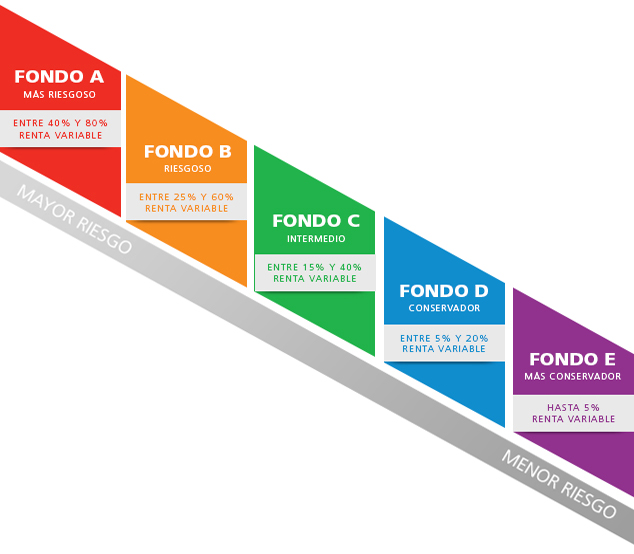
\includegraphics [scale=0.3]{images/multifondos.jpg}
    \caption{Fondo de pensiones}
    
\end{figure}

\chapter{Marco teórico.}
\section{Arquitectura financiera.}
Las administraciones de fondos de pensiones son entidades que tienen el objetivo de capitalizar a largo plazo los activos de una persona. Dicho esto, las formas en que estas operan es mediante el uso de la matemática financiera con el objetivo de interpretar el valor del dinero en el tiempo.
\\[0.2]
Los capitales ganados o perdidos en el tiempo son otorgados mediante el uso del interés, el cual es un índice de rentabilidad porcentual adicional a monto otorgado, este factor en el caso de las AFP y APV están sujetos a factores macroeconómicos independientes de estas entidades, a continuación se enumeraran las mas importantes a considerar:
\begin{itemize}
    \item Inflación.
    \item Crecimiento económico de un país.
    \item Tasa de rentabilidad de las AFP y APV.
    \item Inversiones locales y/o globales.
\end{itemize}
\section{Modelos matemáticos}
A continuación describiremos los términos matemáticos utilizados por las entidades financieras a las cuales las AFP y APV no son ajenas.
\subsection{Valor presente.}
El Valor Presente es una fórmula que nos permite estimar cuál es el valor de hoy que tiene un monto de dinero que no se recibirá ahora sino que en un futuro próximo. A lo cual se necesitara saber cual sera el flujo de dinero a través de los años y las tasas de intereses asociadas a cada periodo. 
\subsection{Valor futuro.}
El valor futuro es una formula que nos permite saber cual será el valor de un monto actual en el futuro (inversión), se observara su comportamiento ante cambios porcentuales.
El Valor Futuro es el valor que tendrá en el futuro un determinado monto de dinero que mantenemos en la actualidad o que decidimos invertir en un proyecto determinado.
\subsection{Anualidad.}
Montos de dinero de distintos periodos llevados a valores anuales al igual que los intereses.

\chapter{Desarrollo}
\section{Problema Planteado.}
Se debe realizar una aplicación que permita estimar o proyectar cuanto dinero dispone una persona afiliada a una AFP al momento de su jubilación, suponiendo que la persona que consulta en la aplicación \textbf{Retirement Simulator} percibe actualmente un sueldo bruto \$X pesos, con edad de Y años que tiene al momento de consultar en la aplicación , además esta persona tiene una esperanza de vida de D años. Adicionalmente, junto con el problema anterior esa misma persona presenta la problemática de querer jubilar con una cantidad de \$T pesos por lo que deberá contratar un APV para cubrir el monto entregado por la AFP.
\\[0.8cm]
A continuación se detallarán las variables que describan el problema que tendrá que resolver la aplicación:
\begin{itemize}
    \item SX: Sexo del cotizante.
    \item EH: Edad en años.
    \item FH: Fecha actual (mes/año).
    \item VFH: Valor total fondos.
    \item SIP: Sueldo imponible.
    \item \%COTO: Porcentaje cotización obligatoria.
    \item \%COTV: Porcentaje cotización obligatoria.
    \item MCOTV: Monto cotización voluntaria.
    \item \%RMEF: Rentabilidad mensual esperada del fondo.
    \item \%CMF: Porcentaje de comisión mensual por movimientos del fondo.
\end{itemize}

\section{Solución Propuesta.}
Realizar un análisis financiero del problema mediante el uso de la matemática financiera con la cual se efectuaran cálculos como valores futuros, valores presentes, porcentaje de intereses asociados a los mercados, anualidades y mensualidades.\\
Para plantear una solución al problema ya mencionado, se esquematizara a priori la posible situación que tendrá que resolver la aplicación.\\

\begin{figure}[H]
    \centering
    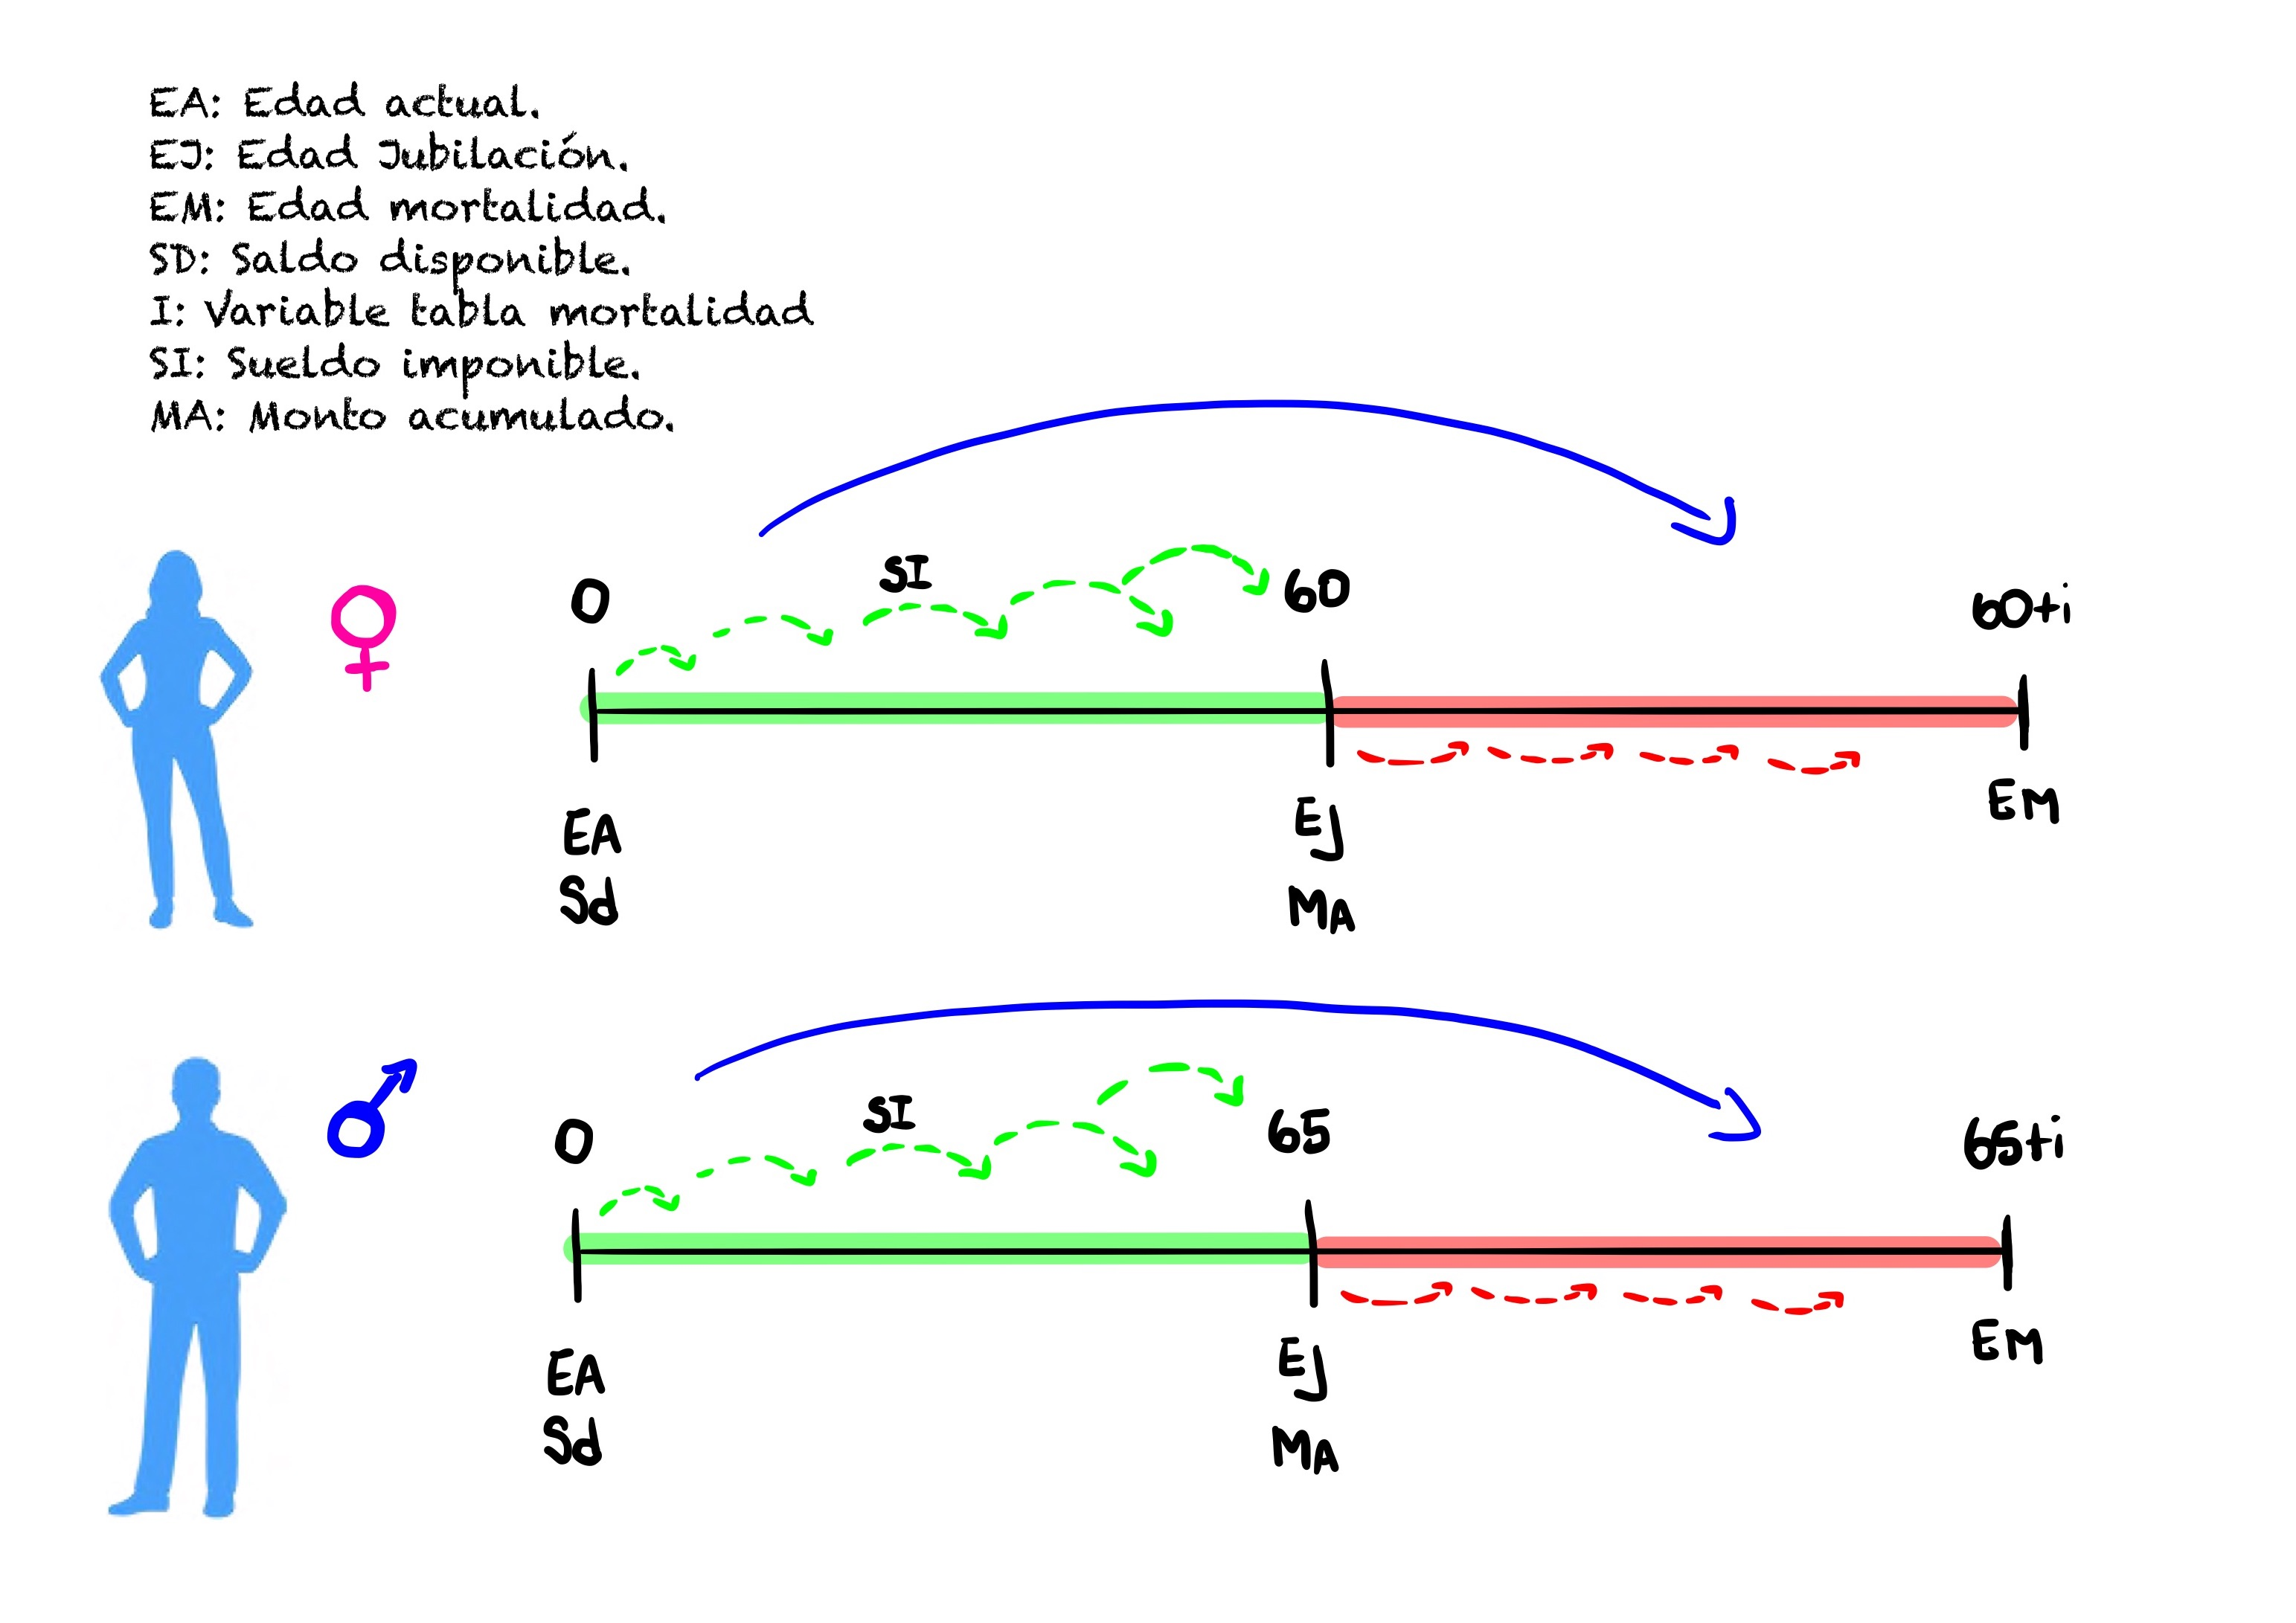
\includegraphics [scale=0.1]{images/afpp.jpg}
    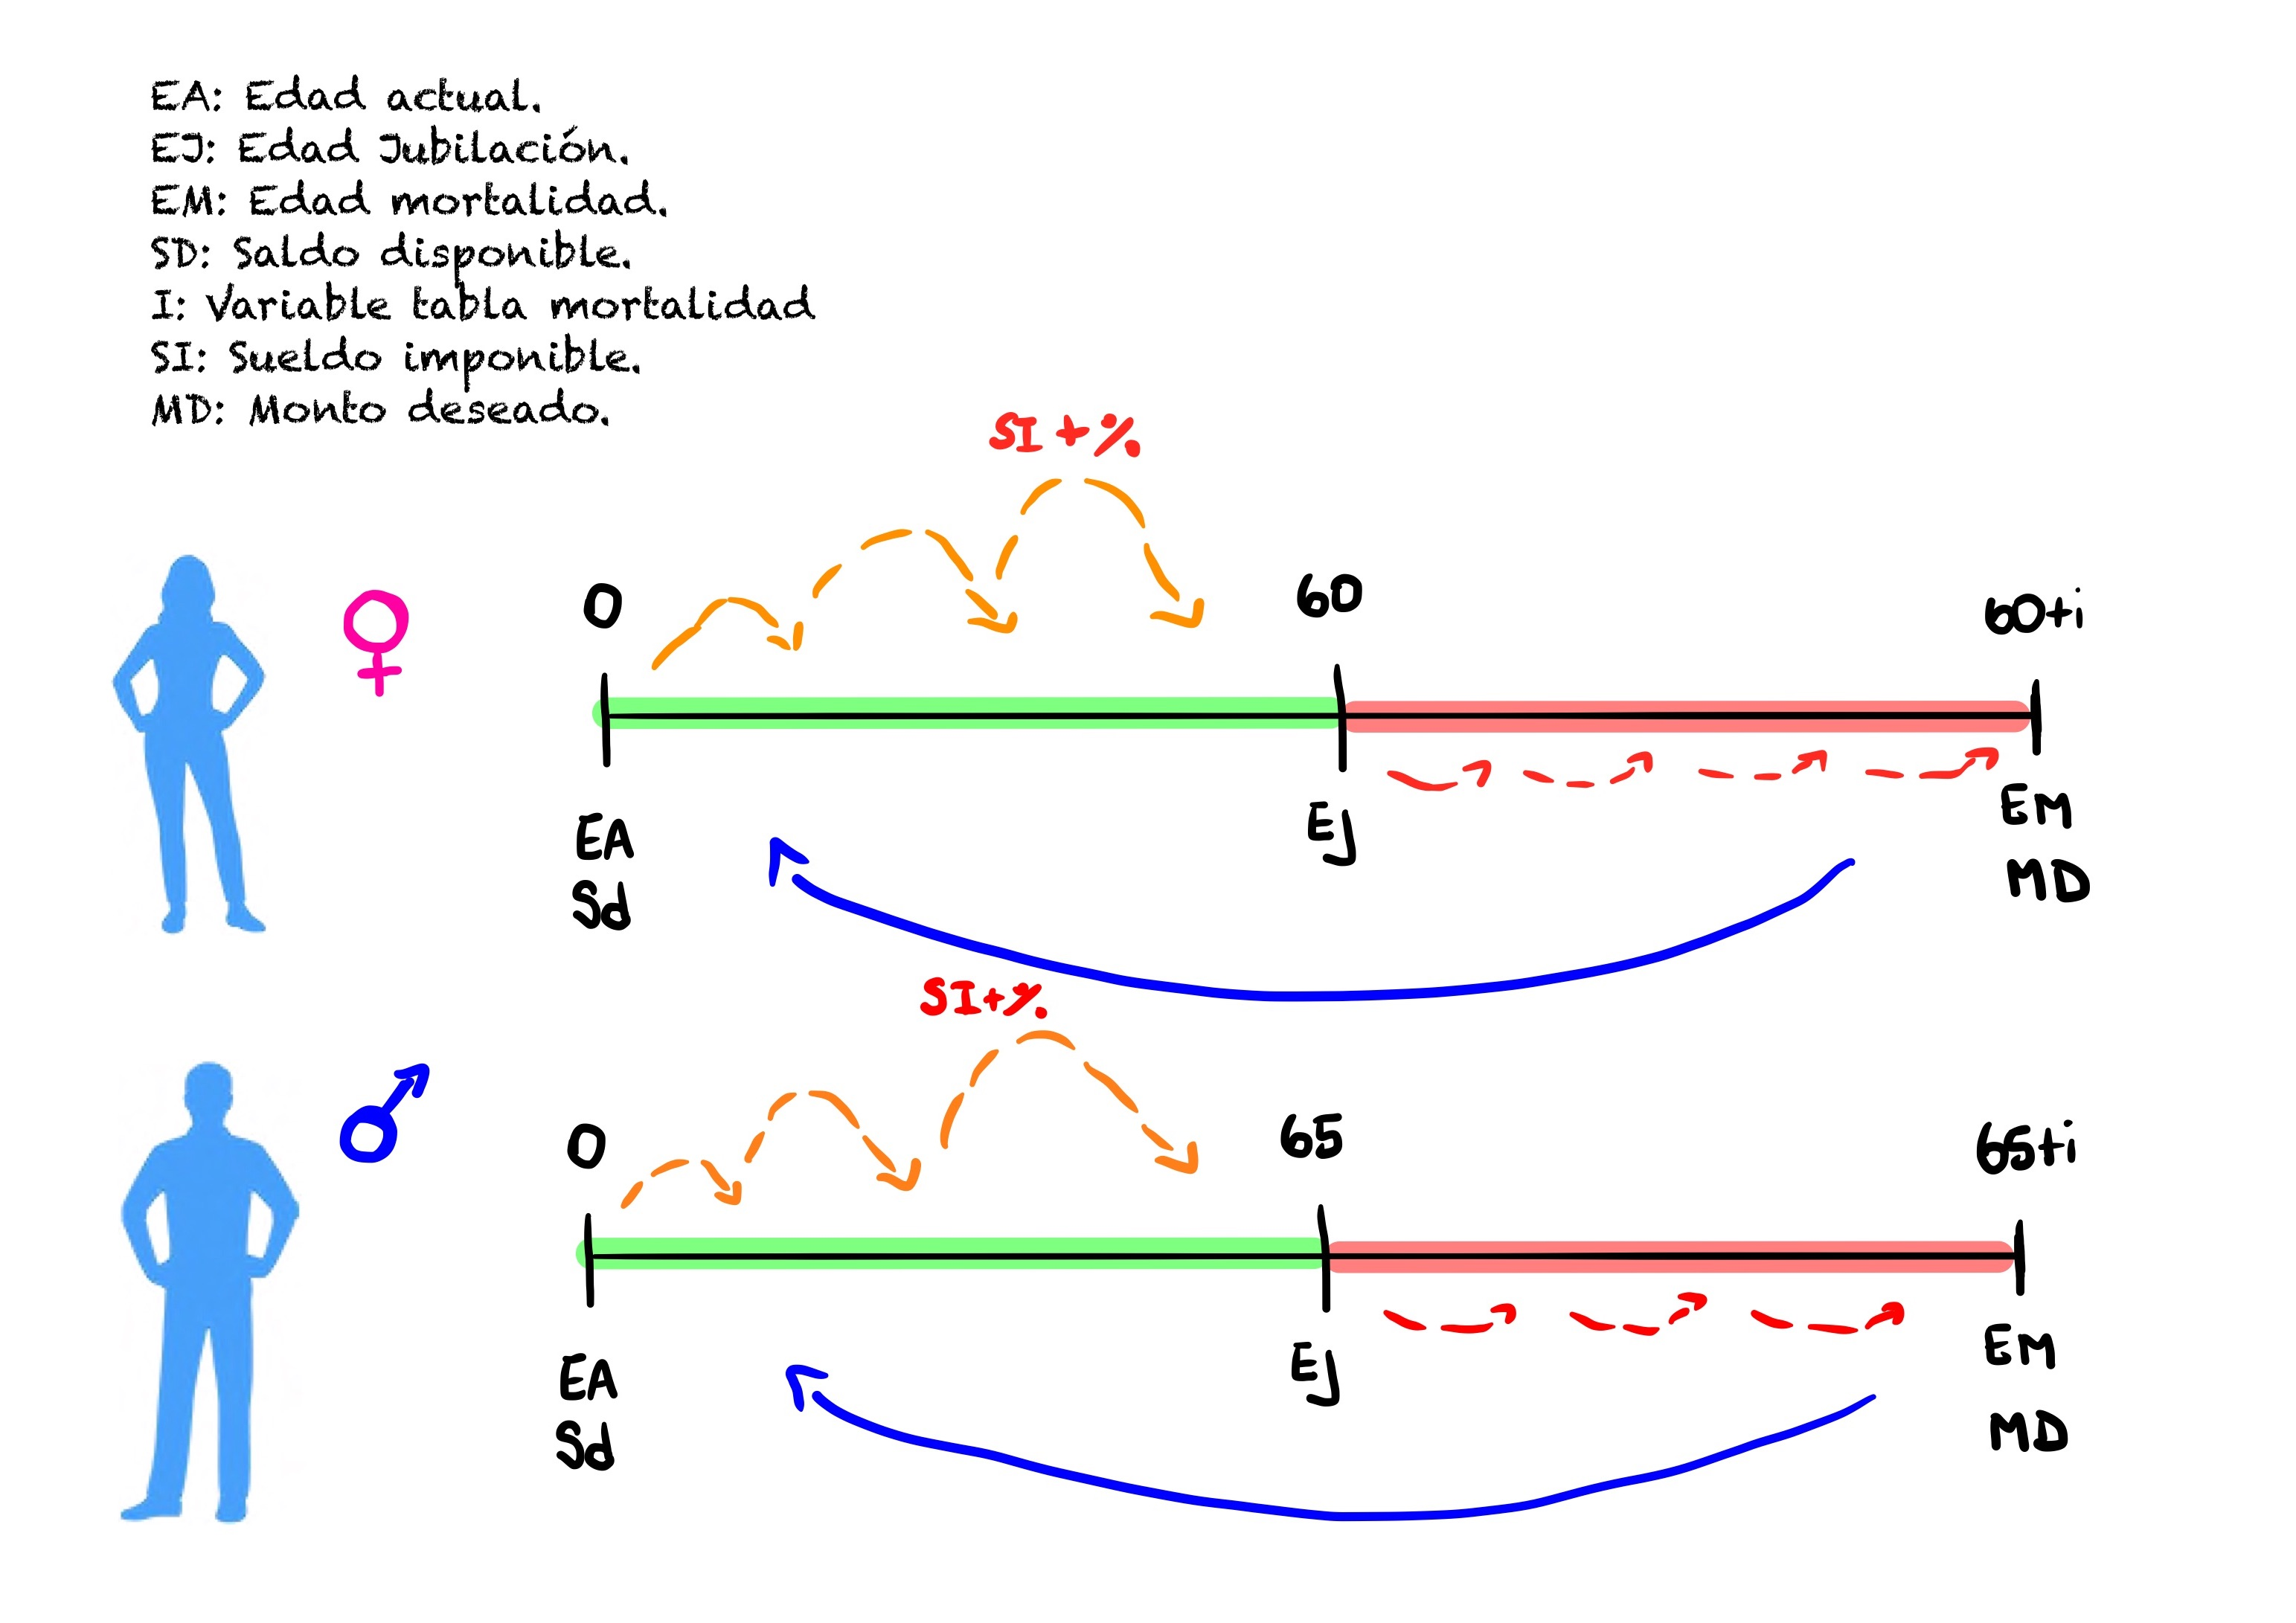
\includegraphics [scale=0.1]{images/apv.jpg}
    
    \caption{AFP y APV}
\end{figure}

Estos estudios deberán ser llevados a la practica mediante el uso de la programación y posteriormente plantearlos mediante una interfaz amigable para el usuario.

\section{Operación y Funcionamiento.}
La aplicación \textbf{Retirement Simulator}, deberá ejecutar un programa que resuelva la situación anteriormente planteada, la interfaz debe ser sencilla antes los ojos del usuario (cotizante) el cual deberá solo ingresar los datos asociados a su sueldo imponible, saldo disponible actualmente en AFP,fecha (mes/año), edad, sexo y su pretensión monetaria al momento de jubilar. \\
En cuanto a la funcionalidad que se desarrollará en la aplicación, le entregaremos al usuario posibles escenarios (conservador, menos conservador, promedio,etc.) el cual esta relacionado al crecimiento real de los sueldos utilizado del índice de remuneraciones por hora entregados por el INE ( instituto nacional de estadística).
\section{Planificación del proyecto.}
Para la planificación del proyecto, se acuerda entre los integrantes del grupo dividir el tiempo de trabajo (en minutos), estimando el nivel de dificultad de cada parte del proyecto y distribuyendo la carga en función de las habilidades más fuertes de cada integrante.
\\

\begin{figure}[H]
    \centering
    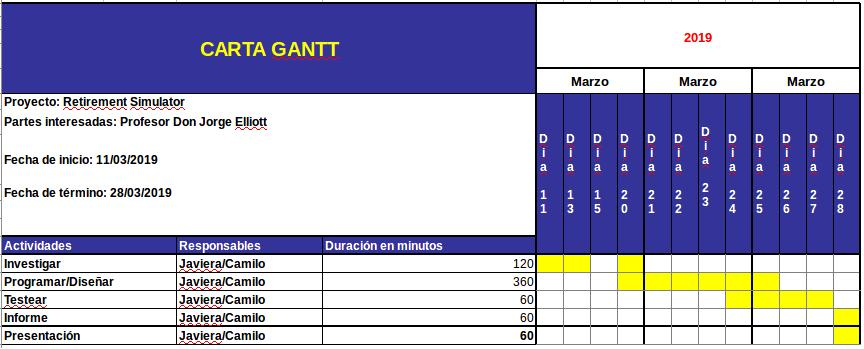
\includegraphics [scale=0.5]{images/cartag.jpg}
    \caption{Carta Gantt.}
    
\end{figure}
\chapter{Formulas y cálculos.}
Para el análisis y el desarrollo de la aplicación, se realizaron cálculos obtenidos de los factores de derivación de pago, con el propósito de obtener los métodos de calculo necesarios para las pensiones estimadas por una persona.
\section{Formulas y cálculos}
\begin{ecuation}
sueldo.anual=0.1*((100-0.95)/100)*sueldo.base*12
\\[10]
tasa.i=(rentabilidad-inflacion)/100
\\[10]
valor.futuro=sueldo.anual*(1+tasa.i)^(edad.jubilacion-edad.actual)
\\[10]
valor.presente=\[
\sum_{i=1}^{45}valor.futuro/(1+tasa.i)^i 
\]
\\[10]
anualidad=(valor.presente)*((tasa.desc*(1+tasa.desc)^(edad.mortalidad-edad.jubilacion))/(1+tasa.desc)^(edad.mortalidad-edad.jubilacion)-1))

\end{ecuation}
\section{Modelamiento.}
\begin{figure}[H]
    \centering
    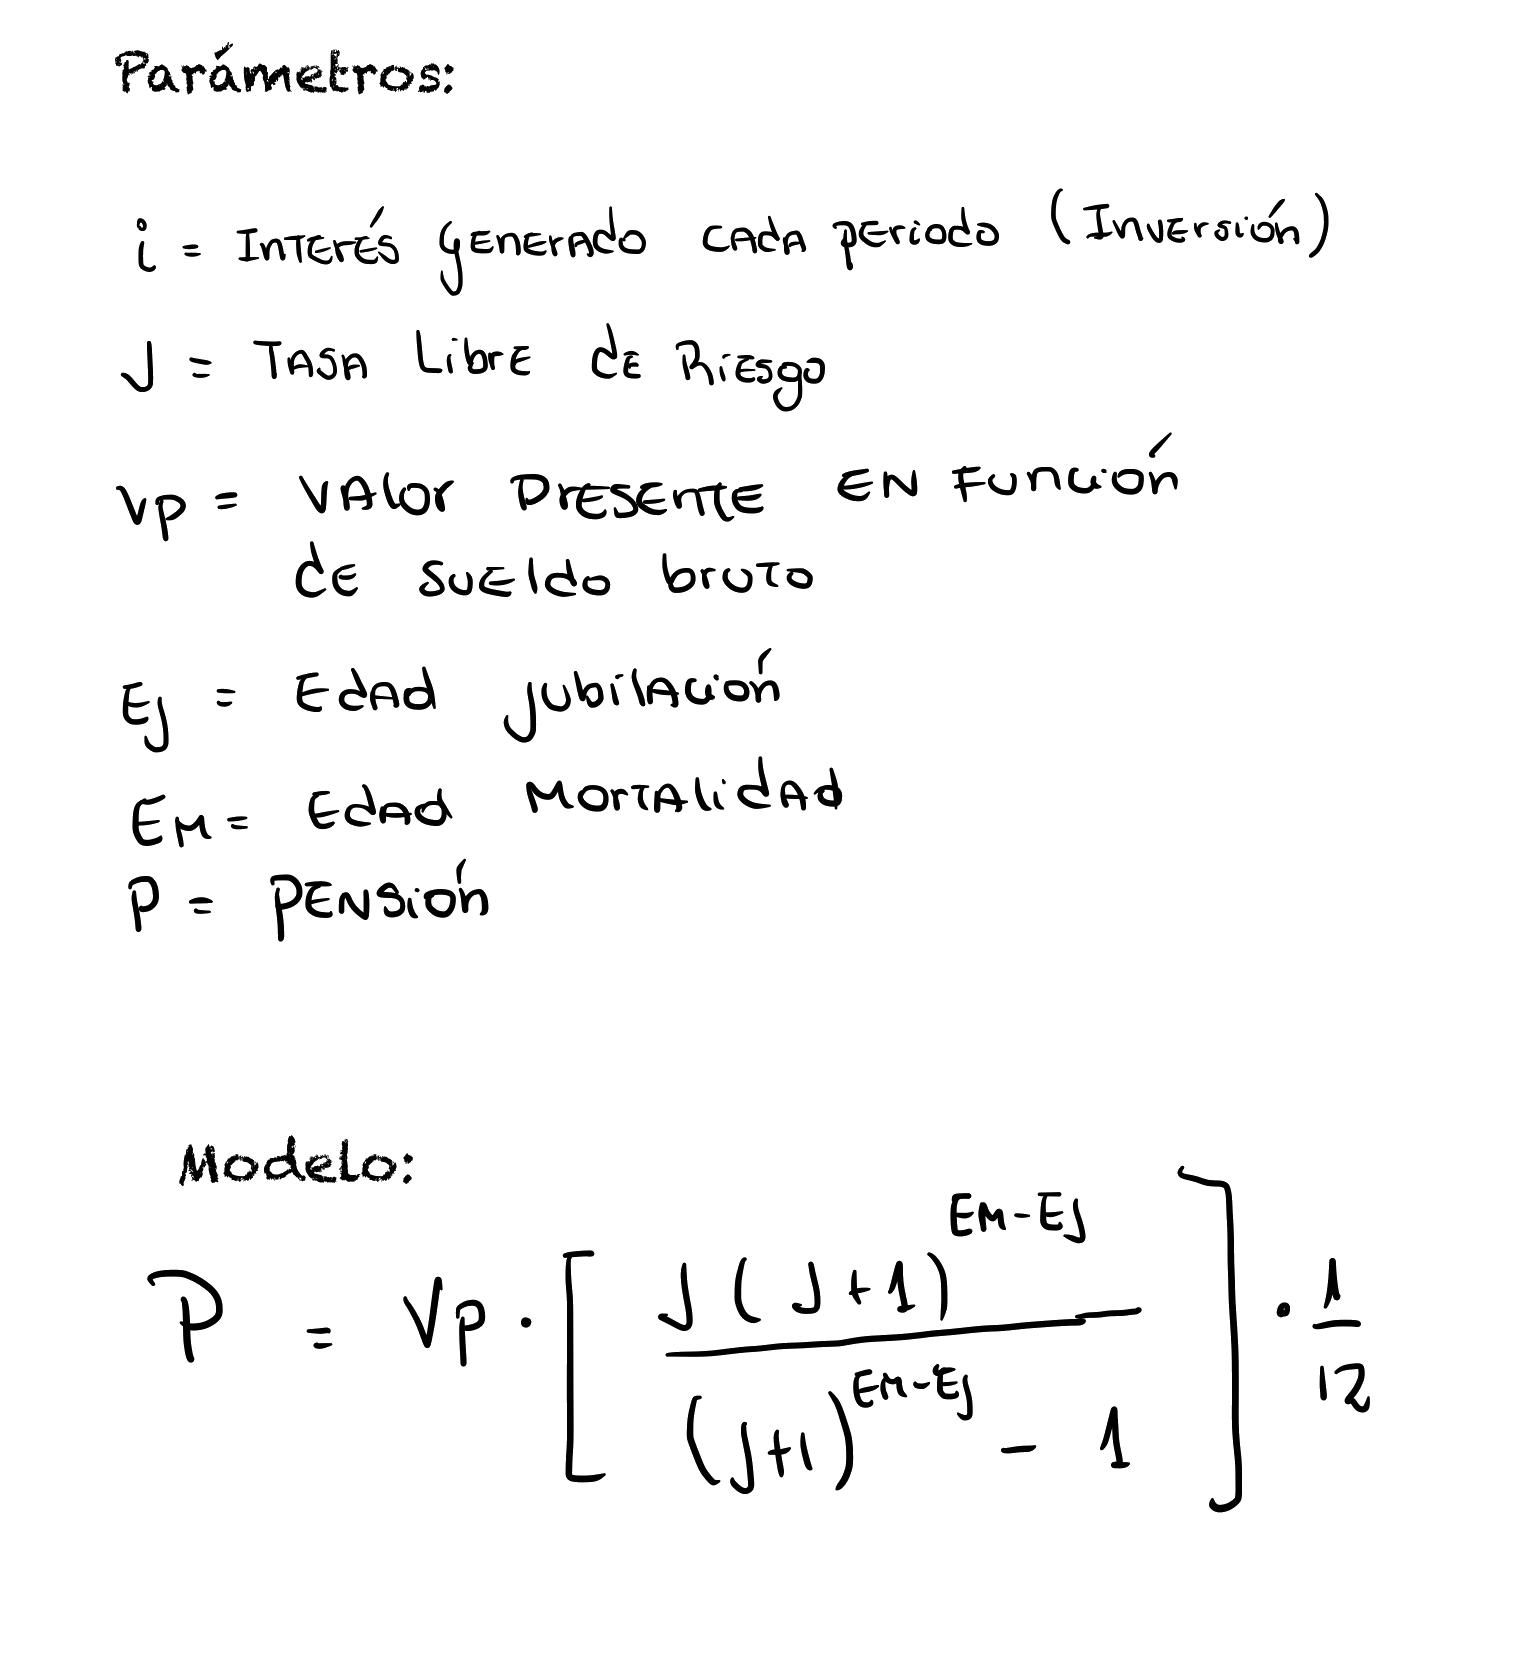
\includegraphics [scale=0.2]{images/modelo1.jpg}
    \caption{Modelo matemático.}
    
\end{figure}
\chapter{Interfaz utilizada para nuestra aplicación.}
\subsection{Arquitectura gráfica.}
Luego de un análisis de cada una de los lenguajes e interfaces existentes en la actualidad, hemos optado por usar HTML5 y CSS3. La razón de esta elección es debido a que la interfaz gráfica otorgada por HTML5 y CSS3  presentan un gran desarrollo en los requerimientos visuales, considerando que es un lenguaje que sigue en proceso de desarrollo por lo que cada vez mas tiene mas prestaciones para los desarrolladores.






\subsection{Arquitectura lógica.}
En cuanto al funcionamiento lógico de nuestra aplicación utilizamos JAVASCRIPT, este lenguaje nos proporciona el manejo  de las ecuaciones matemáticas obtenidas, dando pie al desarrollo y  la ejecución de algoritmos simples. 
\subsection{Solución a lo pedido.}
La integración de los tres lenguajes nos proporciona la solución a lo pedido por nuestra aplicación,  una interfaz amigable de fácil manipulación y de cálculos estimados mas próximos a lo que puede proyectar una persona en su pensión futura.

\begin{figure}[H]
    \centering
    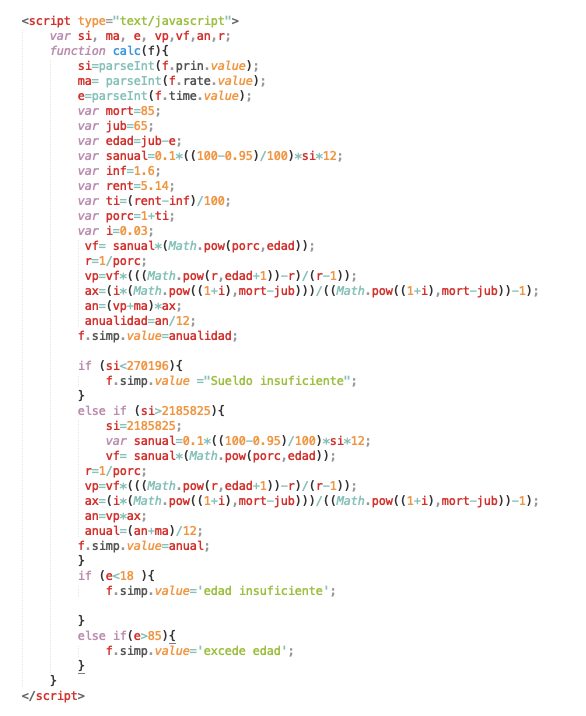
\includegraphics [scale=0.2]{images/afphombre.png}
    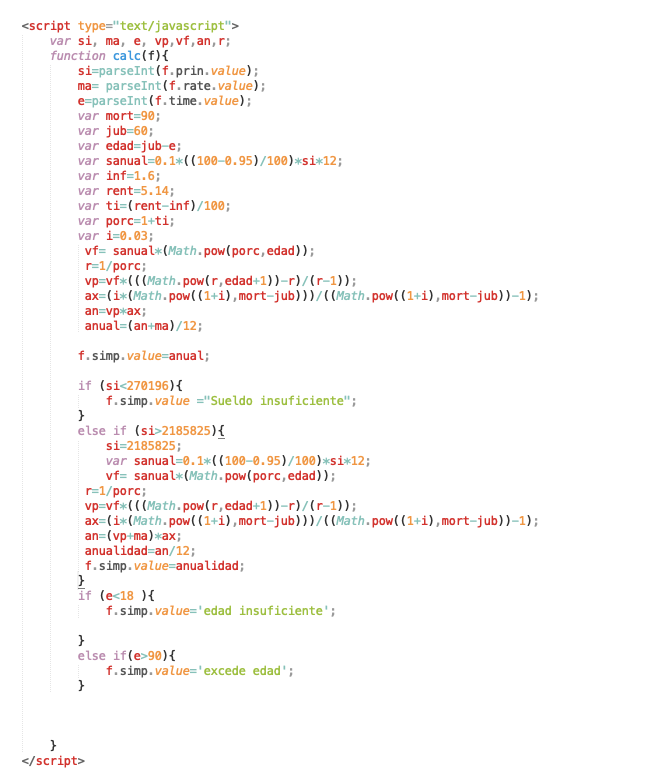
\includegraphics[scale=0.2]{images/afpmujer.png}
    \caption{Modelo matemático.}
    
\end{figure}





\chapter{Conclusiones.}
Con respecto a el desarrollo de la aplicación se pretende preliminarmente trabajar con Javascript para programar el problema planteado, dando el diseño de interfaz sencilla para el cliente con HTML5 y CSS3. 
\\
También se ve la posibilidad del uso de React y Ant Desing para lograr la interfaz deseada.
\\
El objetivo final propuesto por parte de nosotros es realizar un enfoque centrado al problema el cual nos dará como producto la solución a la problemática del calculo de las pensiones proyectadas, por consiguiente nos centramos en replicar el modelo productivo de las 3M (MUDA,MURA y MURI).
\begin{itemize}
    \item MUDA: Nos centramos solamente en realizar una interfaz amigable, útil y óptima. Donde los requerimientos solicitados se entreguen rápidamente, Nuestro beneficio es que no perdimos tiempo en programar en distintos lenguajes y solo nos enfocamos en HTML,CSS3 y JS.
    \item MURA: De un análisis de las fortalezas y debilidades de cada uno de los integrantes, nos enfocamos en asignar las tareas orientadas a las fortalezas formando sinergia en el sistema global de trabajo.
    \item MURI: Al asignar las tareas orientadas a las fortalezas bajamos las sobrecargas e ineficiencias en los tiempos de diseño e implementación de la aplicación.
\end{itemize}
Debemos destacar que la implementación de nuestra aplicación no solo nos ayudo a ver como debemos abordar la realización de un proyecto si no que también al problema que existe actualmente sobre las pensiones en Chile. Como grupo nos propusimos la realización de este proyecto lo mas parecido a la realidad por lo que esperamos que sea de gran utilidad para quienes lo utilicen.

\chapter{Bibliografía.}
\begin{itemize}
    \item Documento de estudio "AFP, pensiones y modificaciones", José Parada Daza.
    \item https://www.ine.cl/
    \item https://www.spensiones.cl
    \item Ingeniería económica, Lelant T.Blank y A.J Tarquin.
    \item Preparación y evaluación de proyectos, Nassir Sapag Chain y Reinaldo Sapag Chan.
\end{itemize}

\end{document}
